\begin{figure}
	\centering
	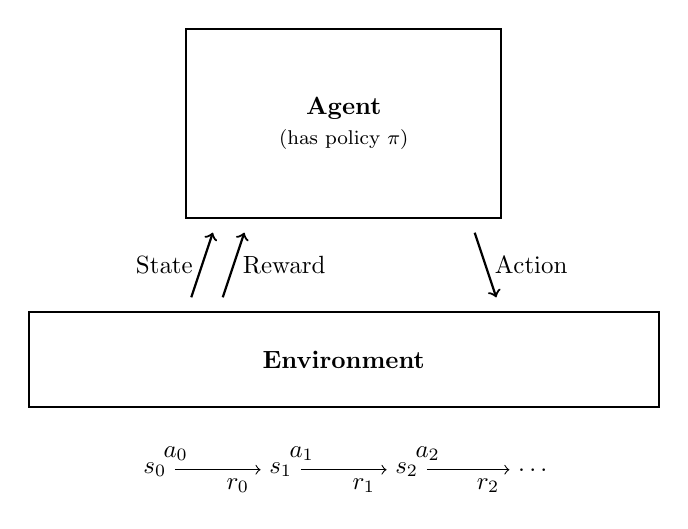
\begin{tikzpicture}[
		scale=0.4,
		every node/.style={scale=0.9}
	]
	
		\draw[thick] (0,0) -- (20,0) -- (20,3) -- (0,3) -- cycle;
		\node at (10,1.5) {\textbf{Environment}};

		\draw[thick] (5,6) -- (15,6) -- (15,12) -- (5,12) -- cycle;
		\node[align=center] at (10,9) {\textbf{Agent} \\ \footnotesize(has policy $\pi$)\normalsize};

		\draw[shorten >=0.2cm,shorten <=0.2cm,->,thick] (5,3) -- node[left] {State} (6,6);
		\draw[shorten >=0.2cm,shorten <=0.2cm,->,thick] (6,3) -- node[right] {Reward} (7,6);
		\draw[shorten >=0.2cm,shorten <=0.2cm,->,thick] (14,6) -- node[right] {Action} (15,3);

		\node (s0) at (4,-2) {$\bm{s_0}$};
		\node (s1) at (8,-2) {$\bm{s_1}$};
		\node (s2) at (12,-2) {$\bm{s_2}$};
		\node (s3) at (16,-2) {$\dots$};

		\draw[->] (s0) node[above right] {$a_0$} -- node[below right] {$r_0$} (s1);
		\draw[->] (s1) node[above right] {$a_1$} -- node[below right] {$r_1$} (s2);
		\draw[->] (s2) node[above right] {$a_2$} -- node[below right] {$r_2$} (s3);
	
	\end{tikzpicture}
\end{figure}